%Partie discrétisation

First, the method uses discritised observations as an input, thus it is necessary to use an other method which transforms the analogic time series data to discritised time series data.

\begin{figure}
\hspace{-1cm}
\begin{minipage}[t]{0.4\linewidth}
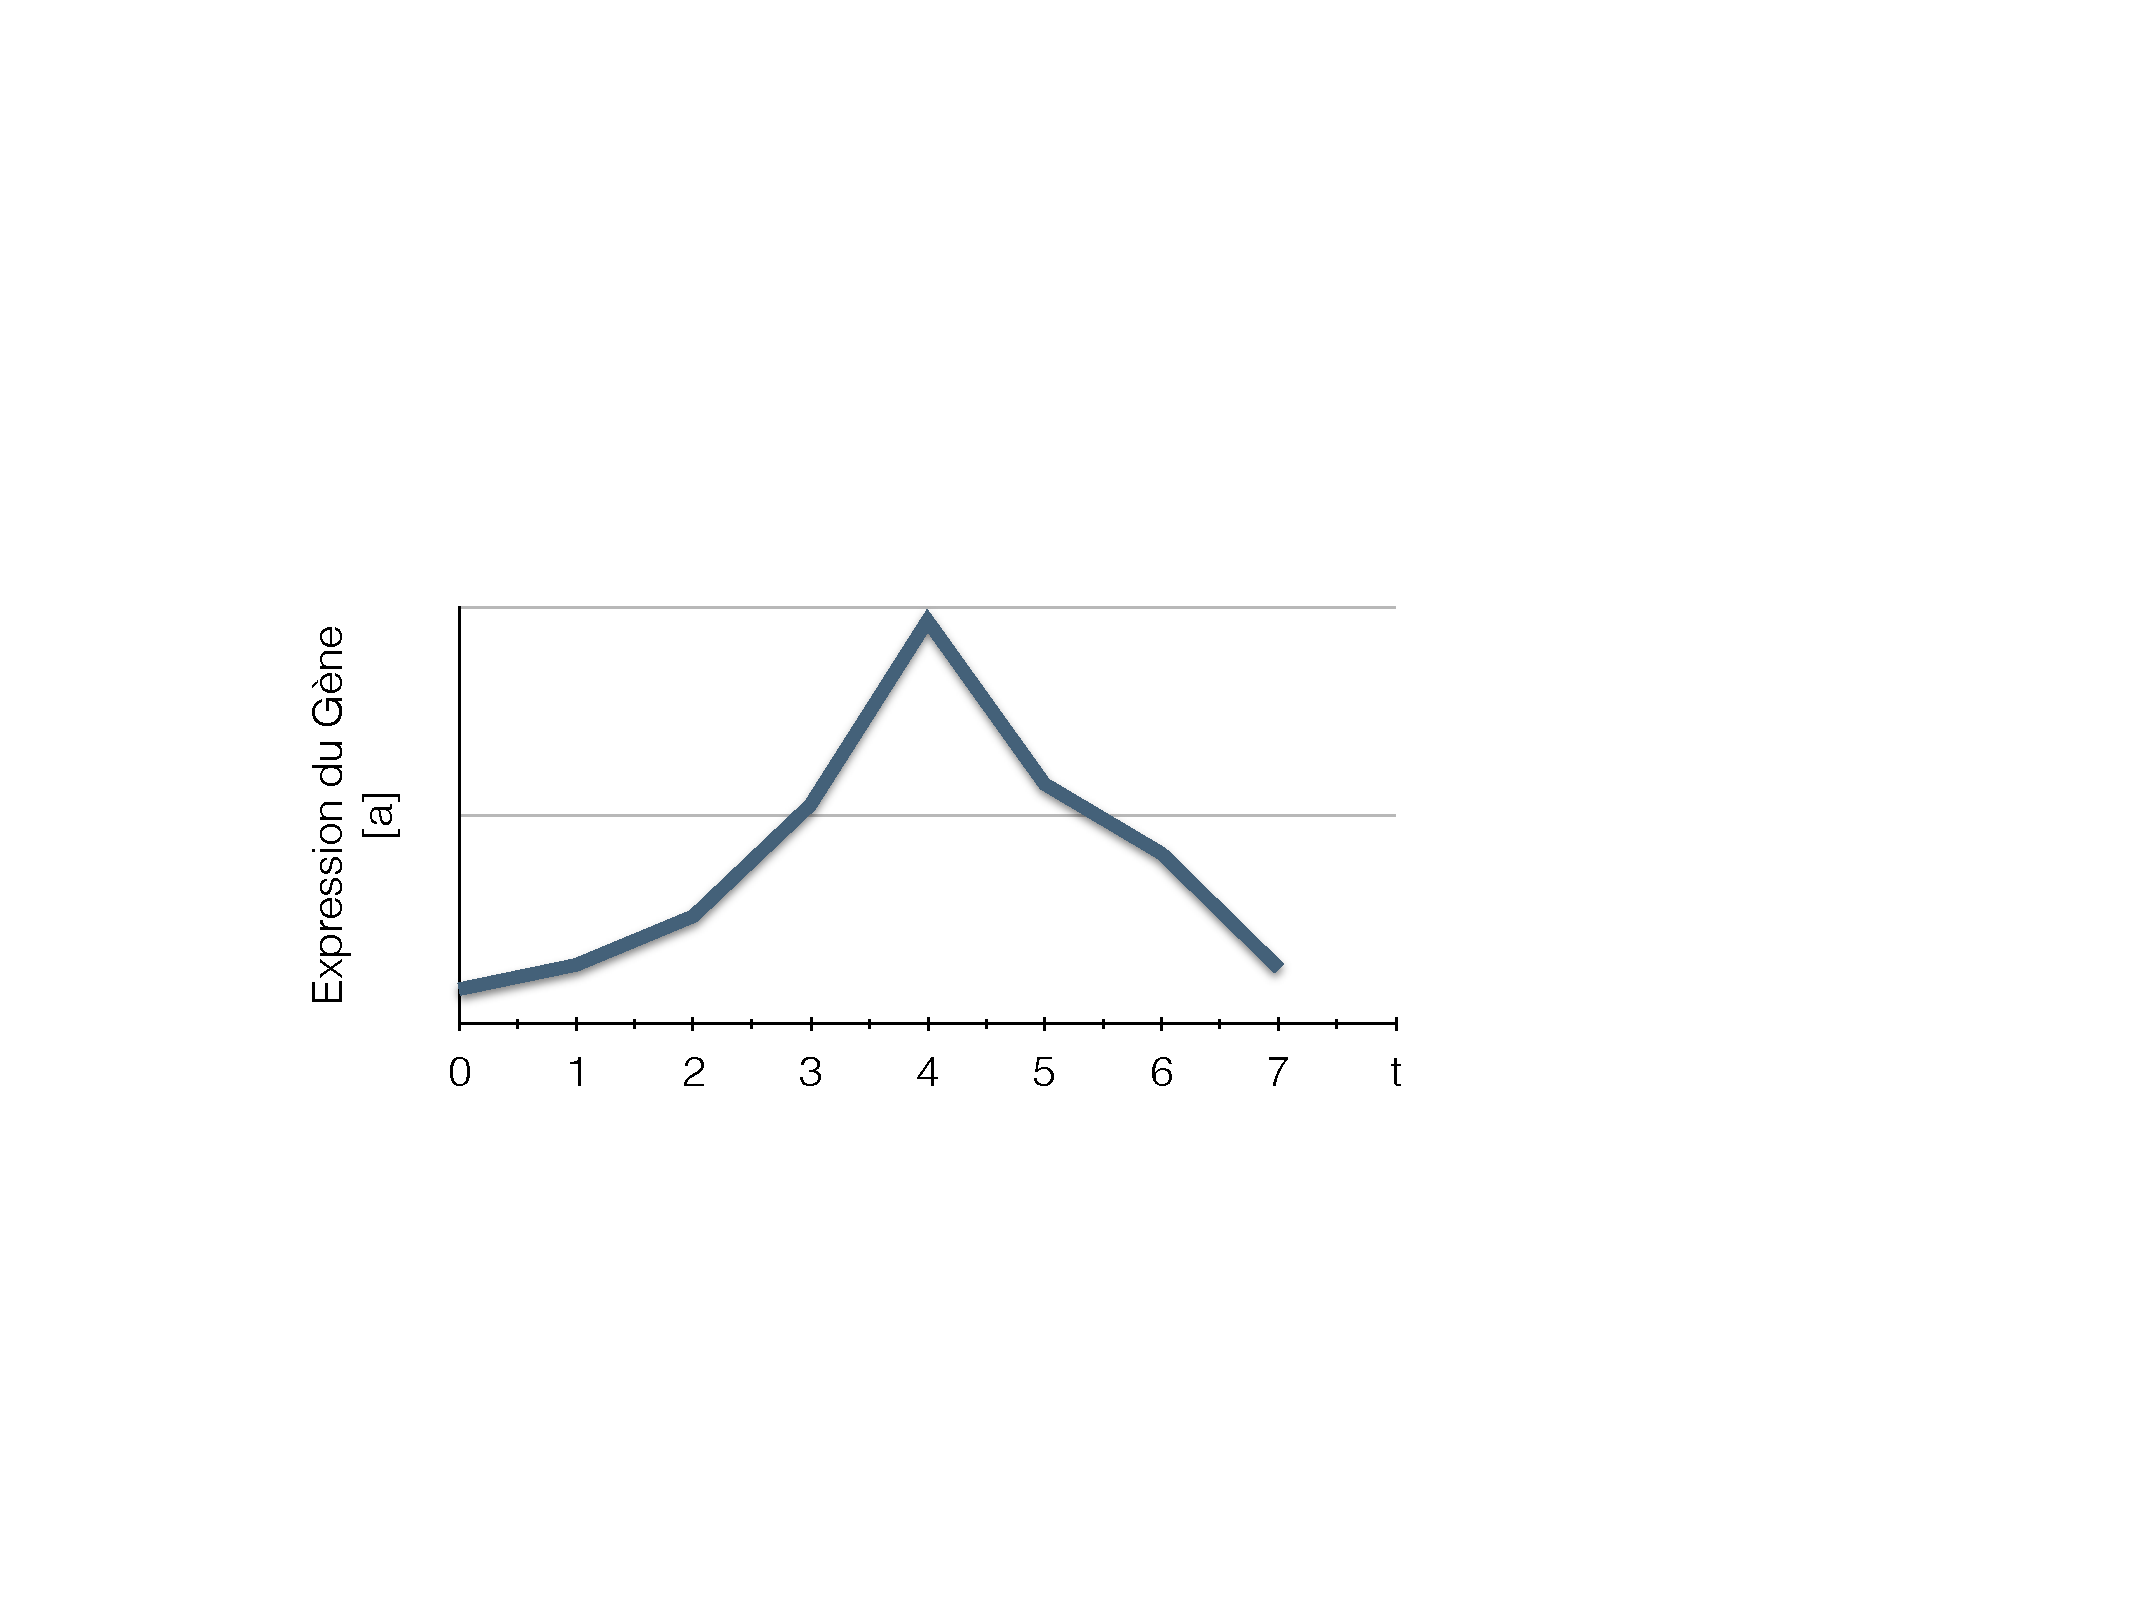
\includegraphics[ width =1\linewidth]{images/courbes/gene-a.pdf}\\
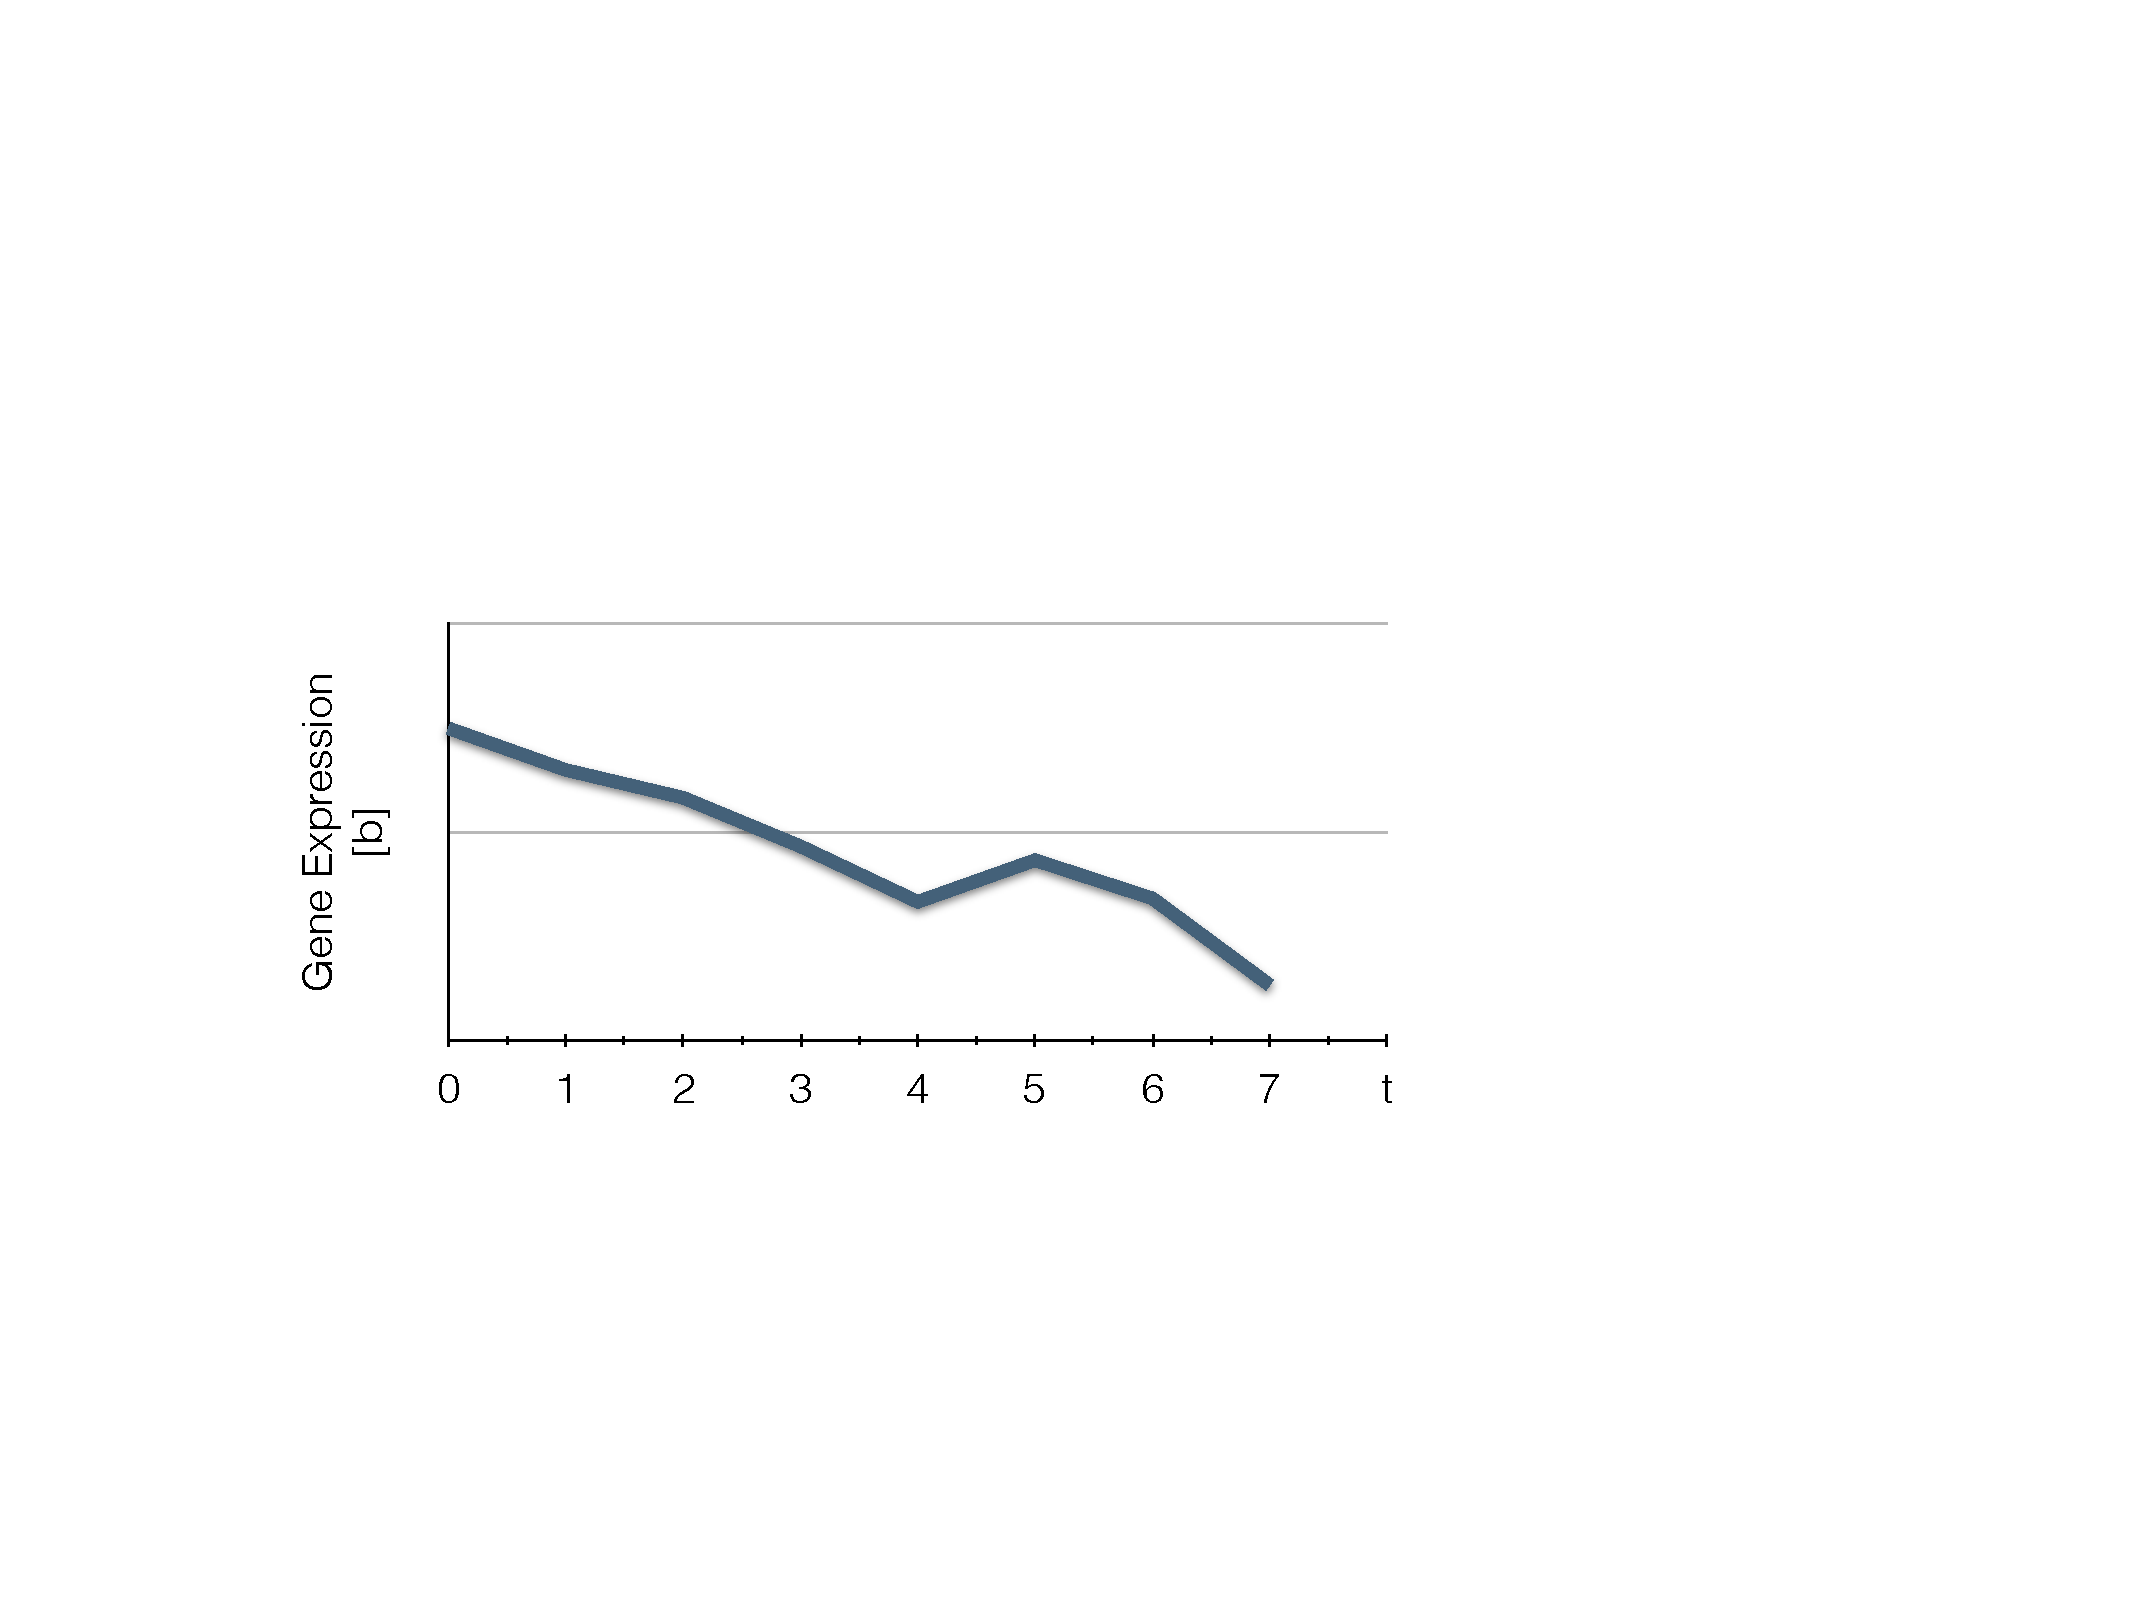
\includegraphics[ width =1\linewidth]{images/courbes/gene-b.pdf}\\
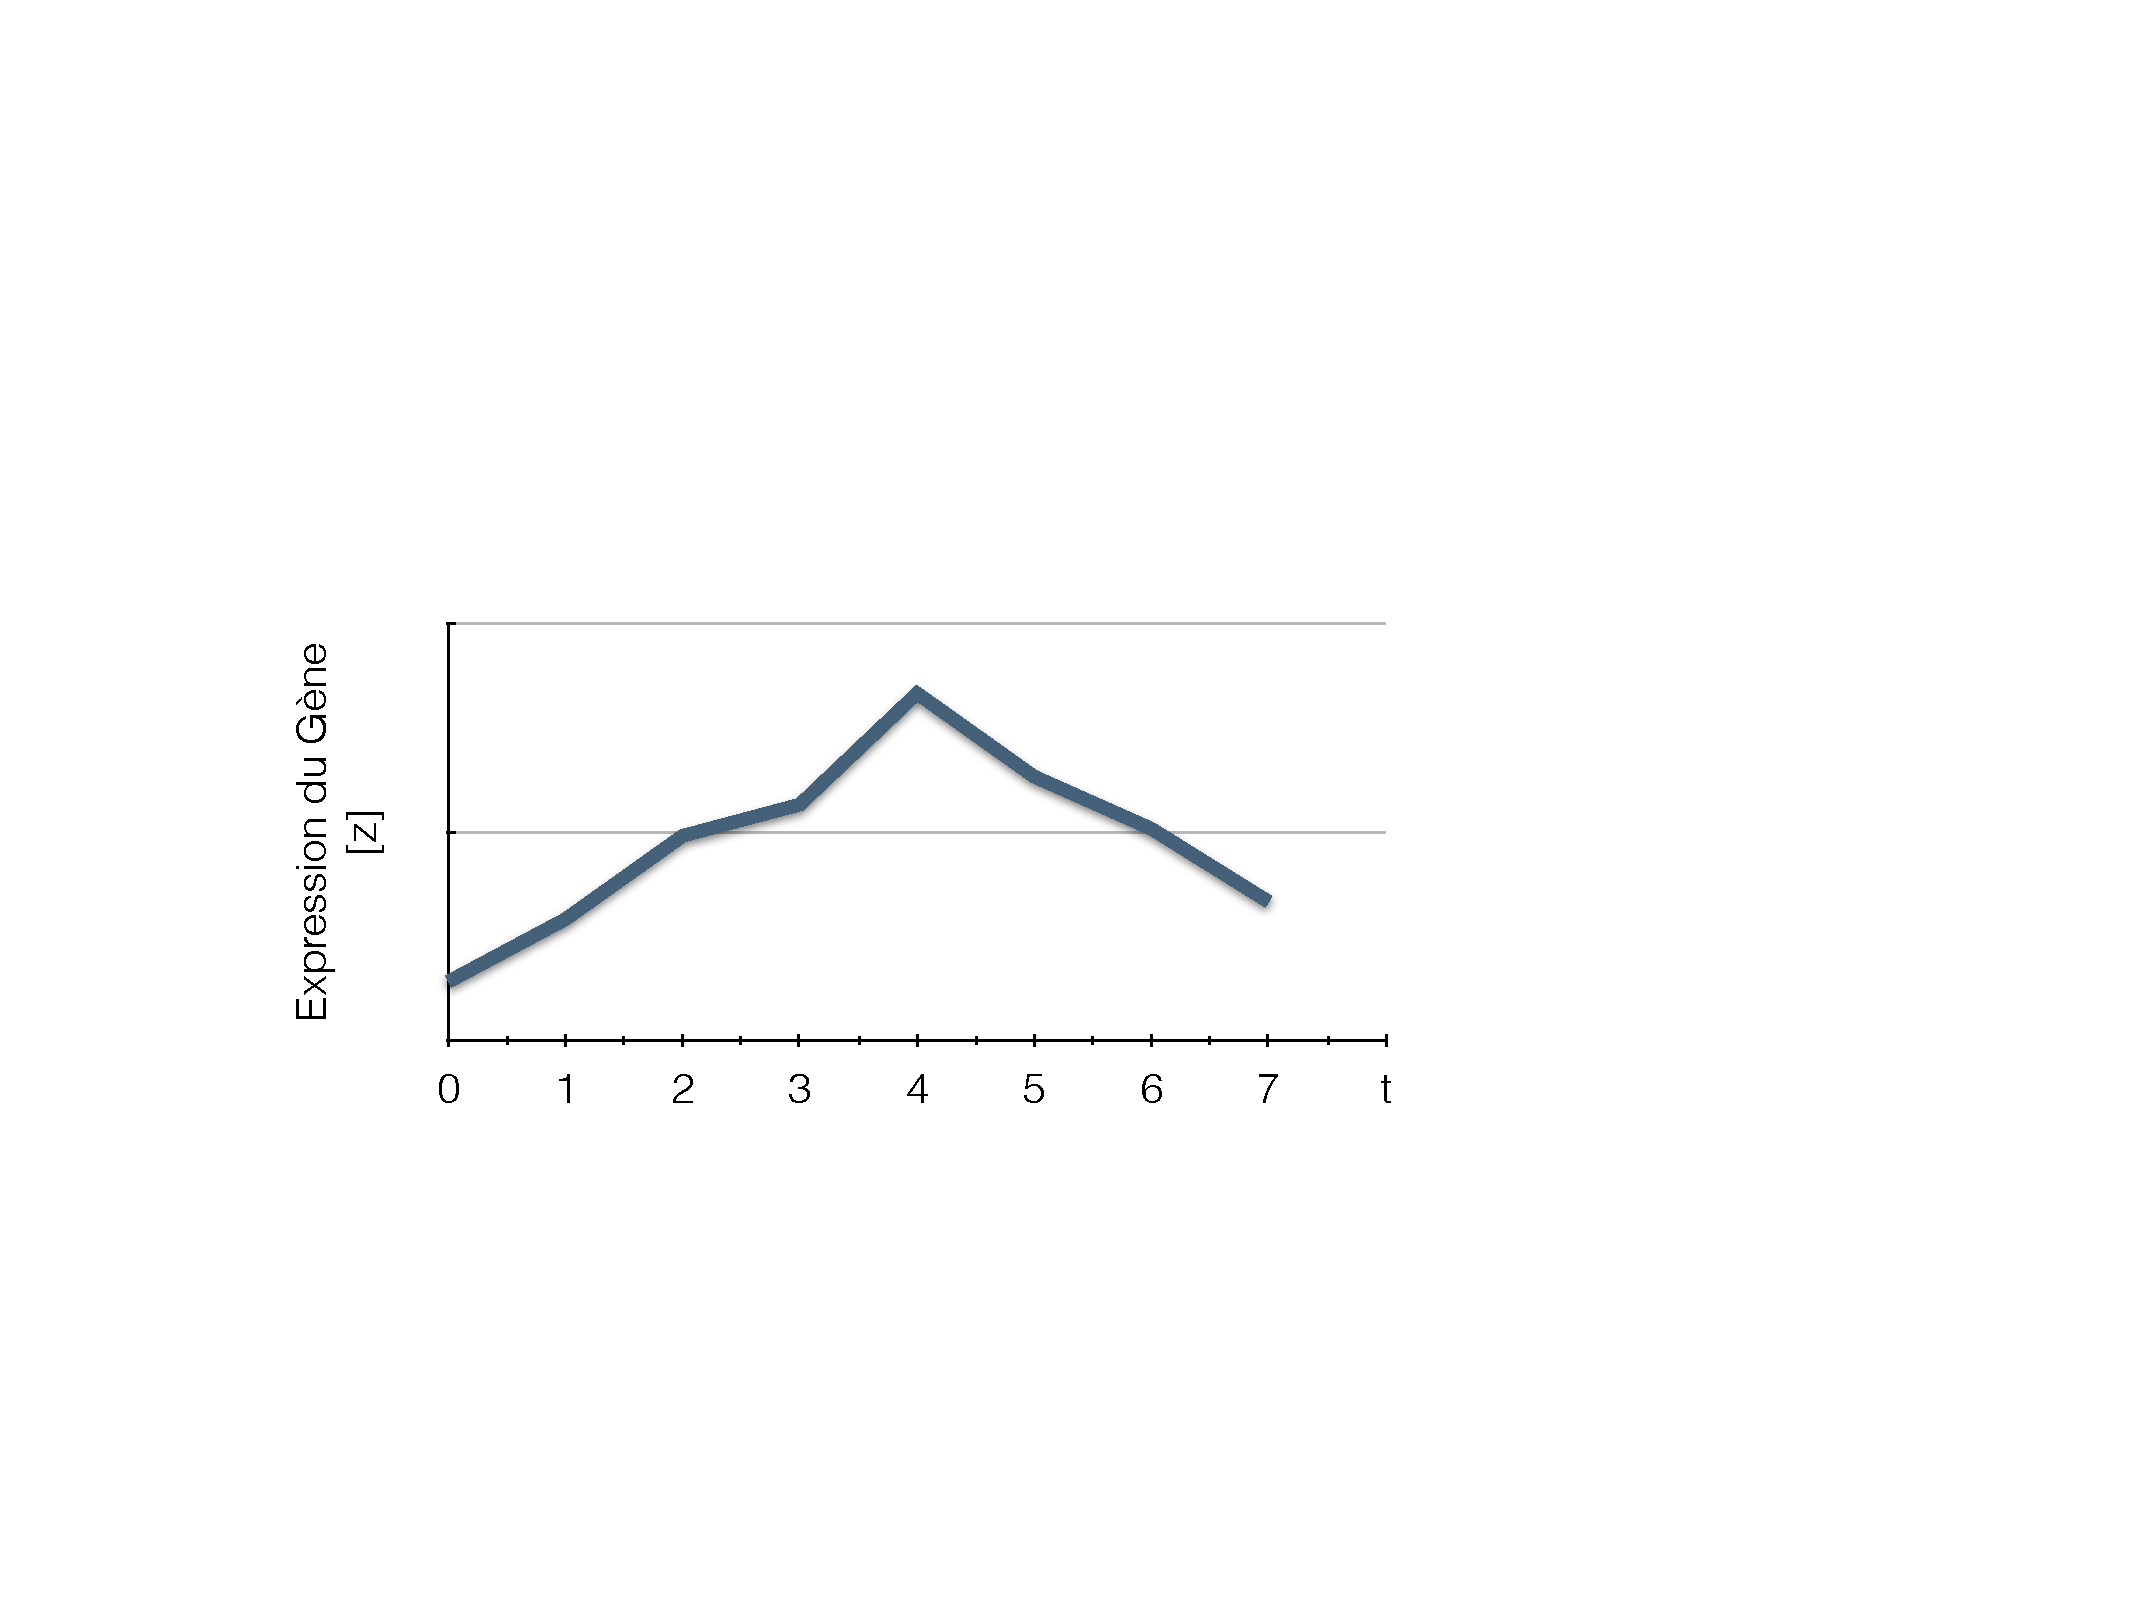
\includegraphics[ width =1\linewidth]{images/courbes/gene-z.pdf}\\
\end{minipage}
\hspace{0.01cm}
\textbf{Discrétisation}
\hspace{0.01cm}
\begin{minipage}[t]{0.4\linewidth}
\centering
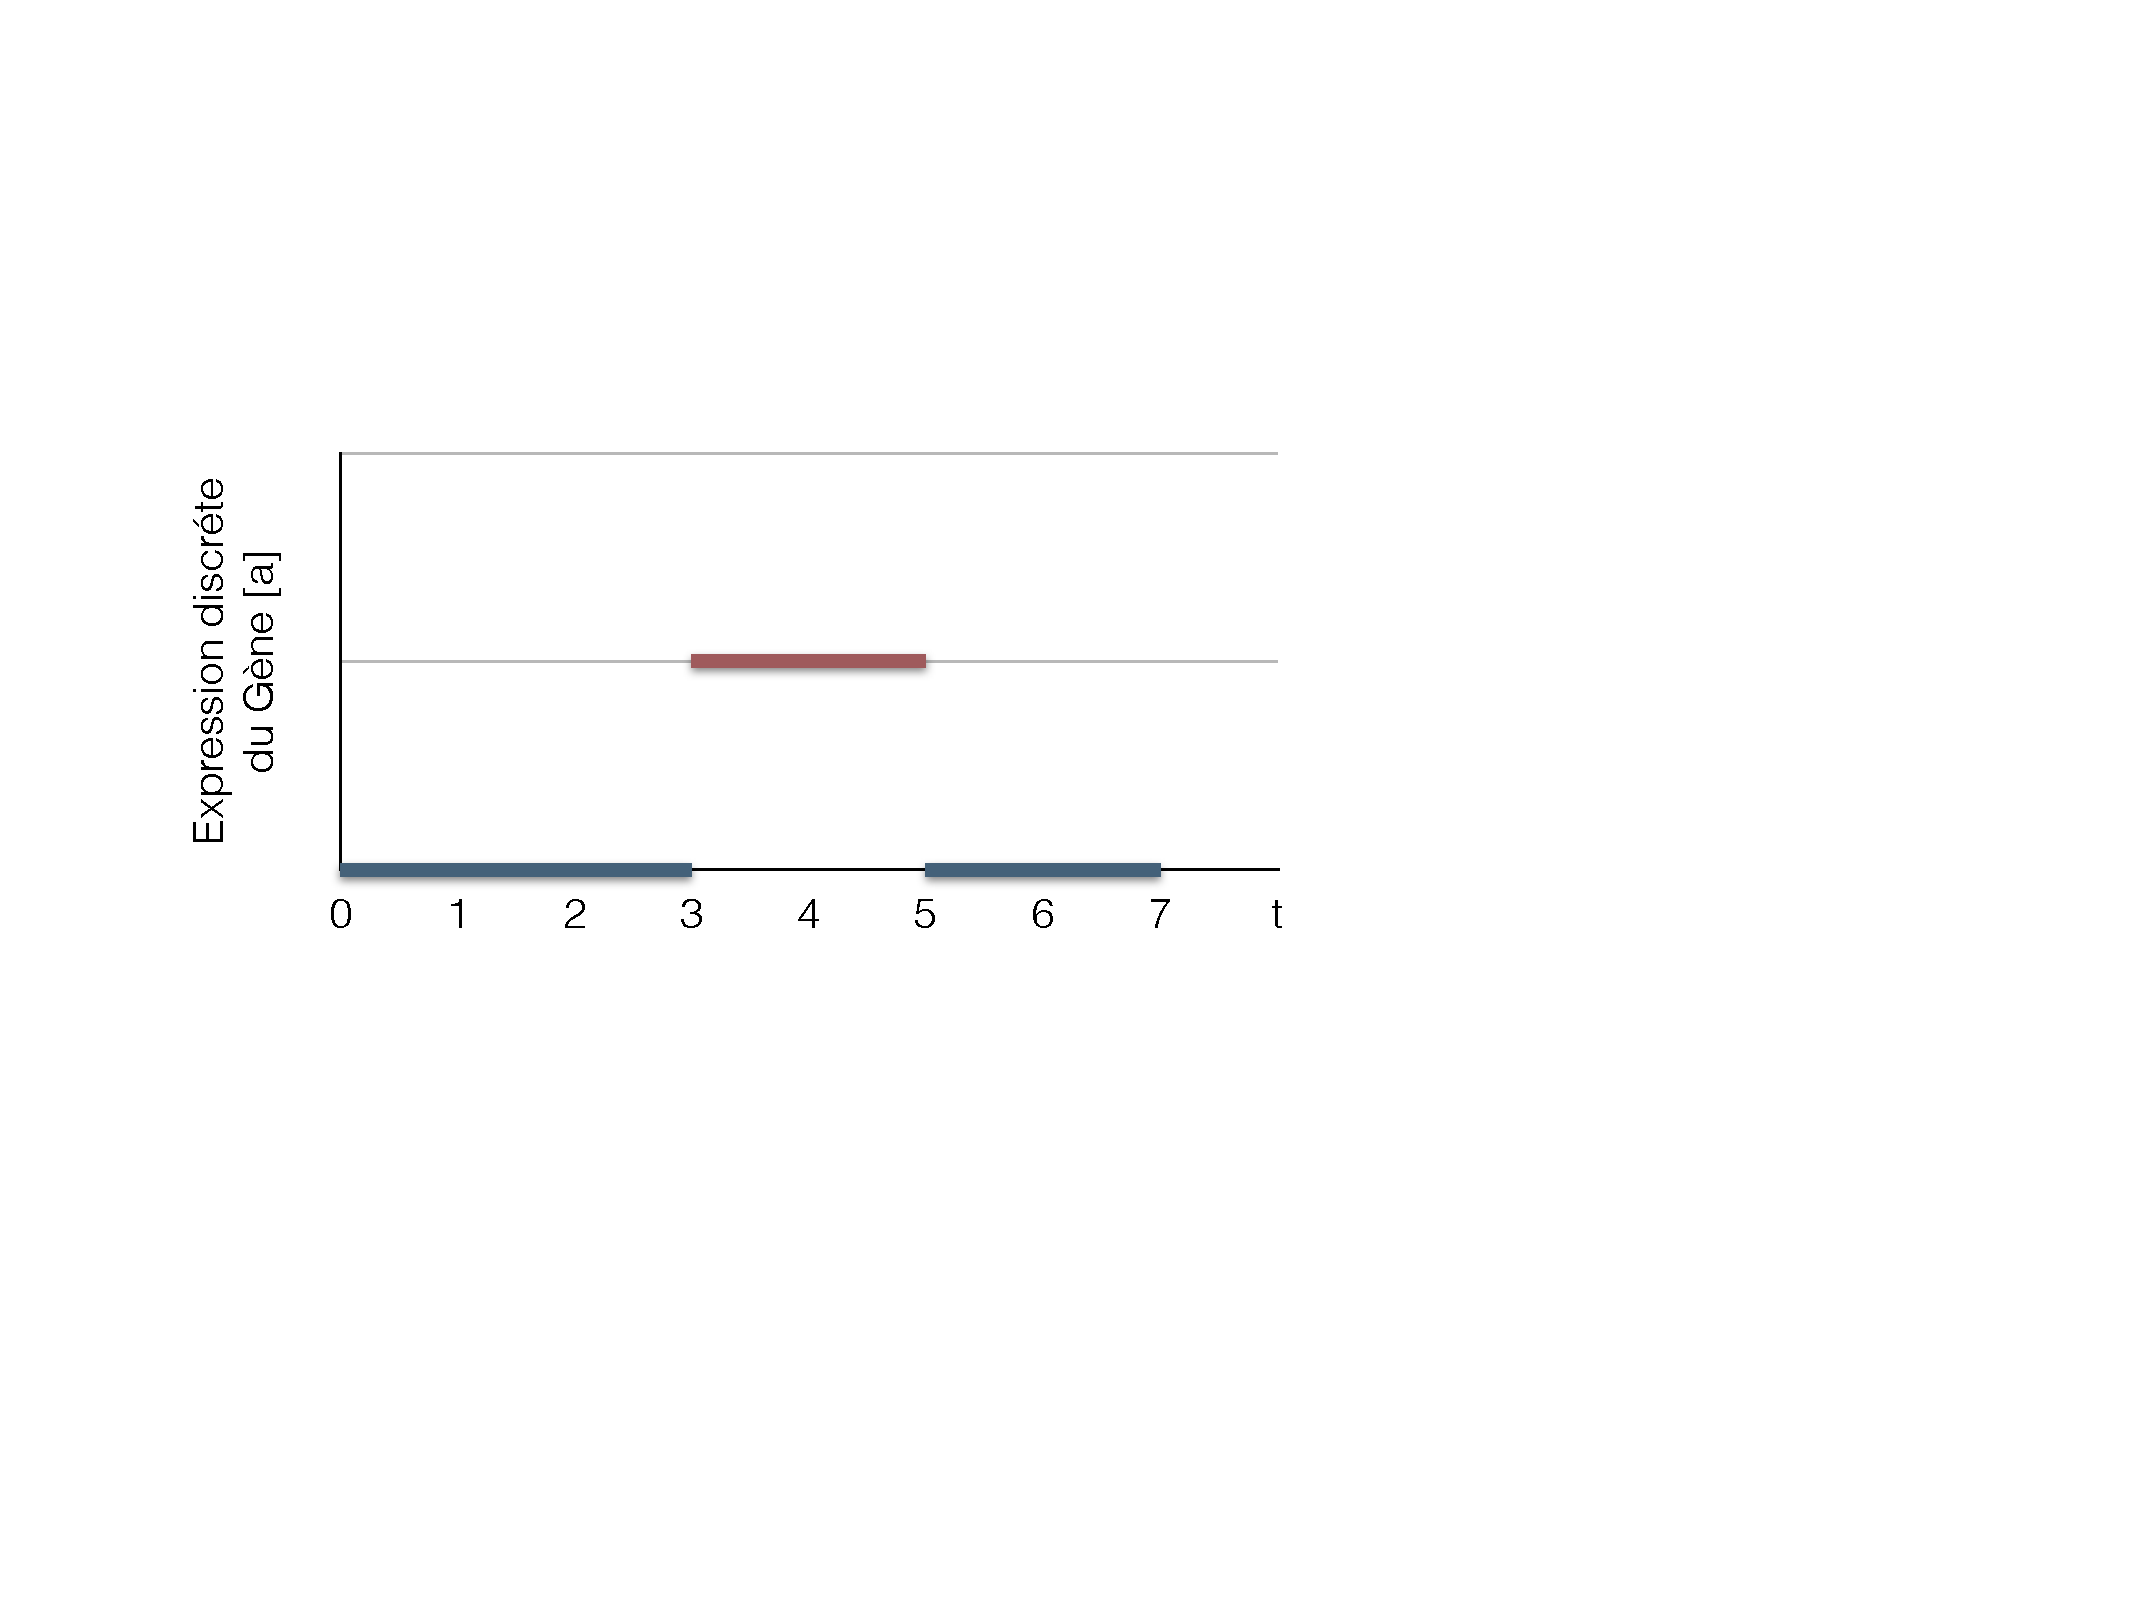
\includegraphics[ width =1\linewidth]{images/courbes/gene-a-disc.pdf}\\
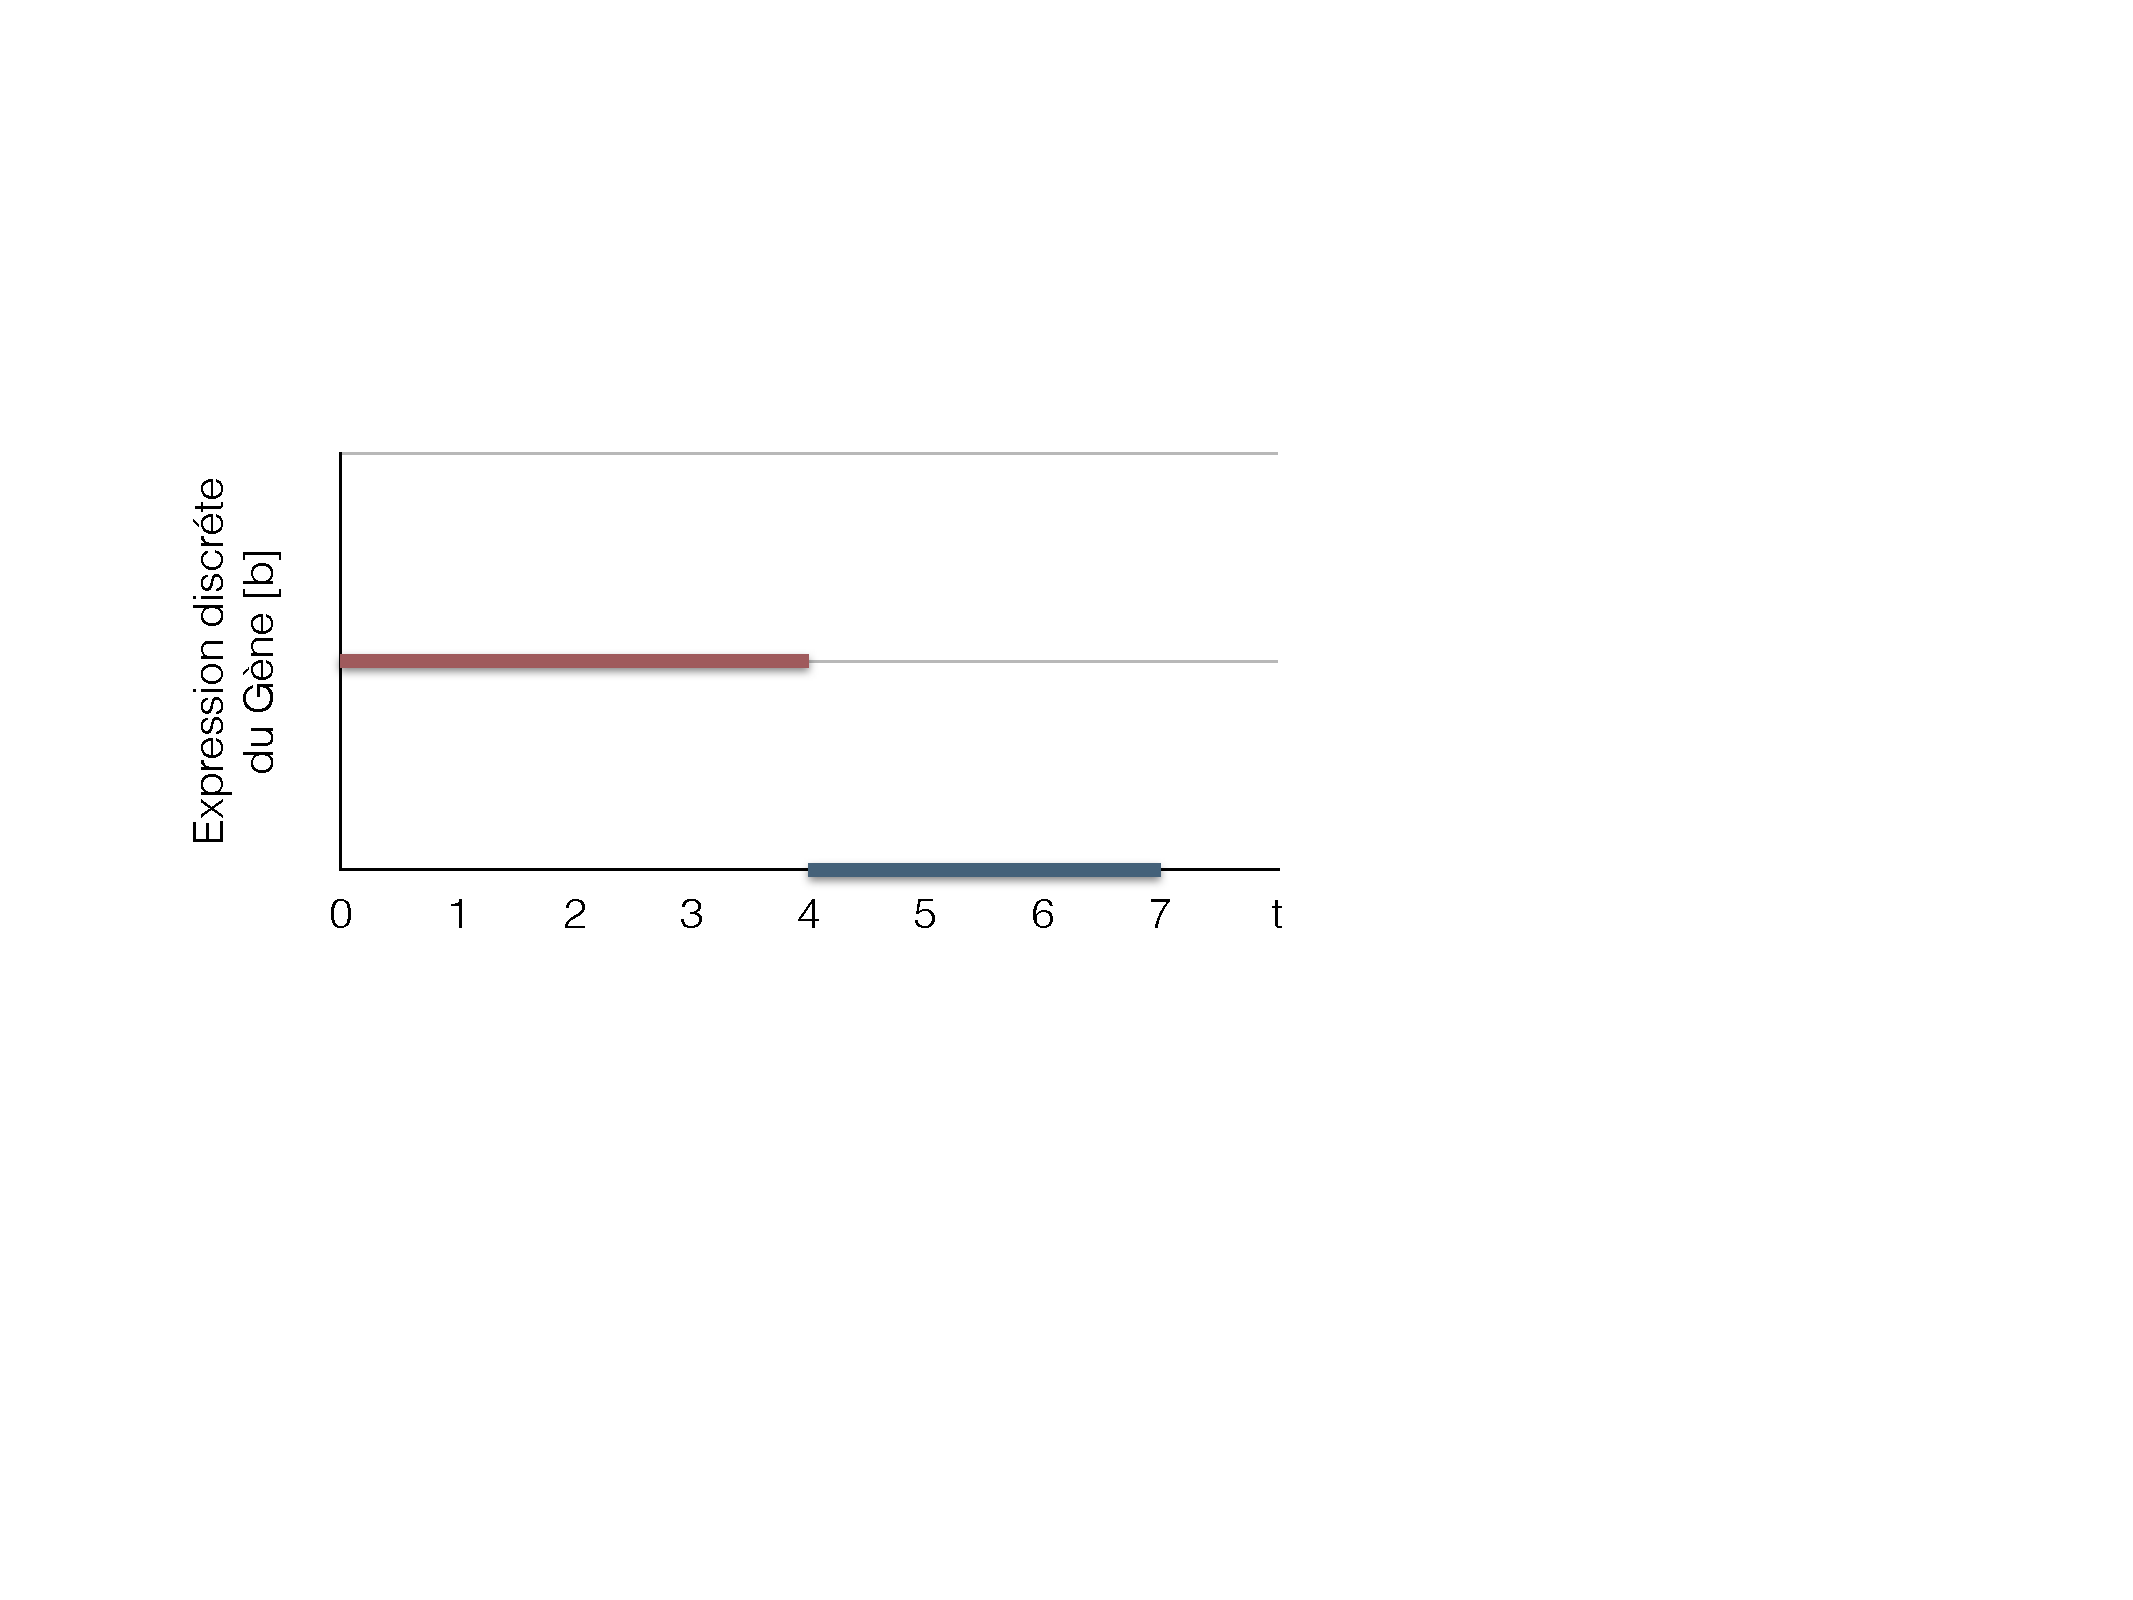
\includegraphics[ width =1\linewidth]{images/courbes/gene-b-disc.pdf}\\
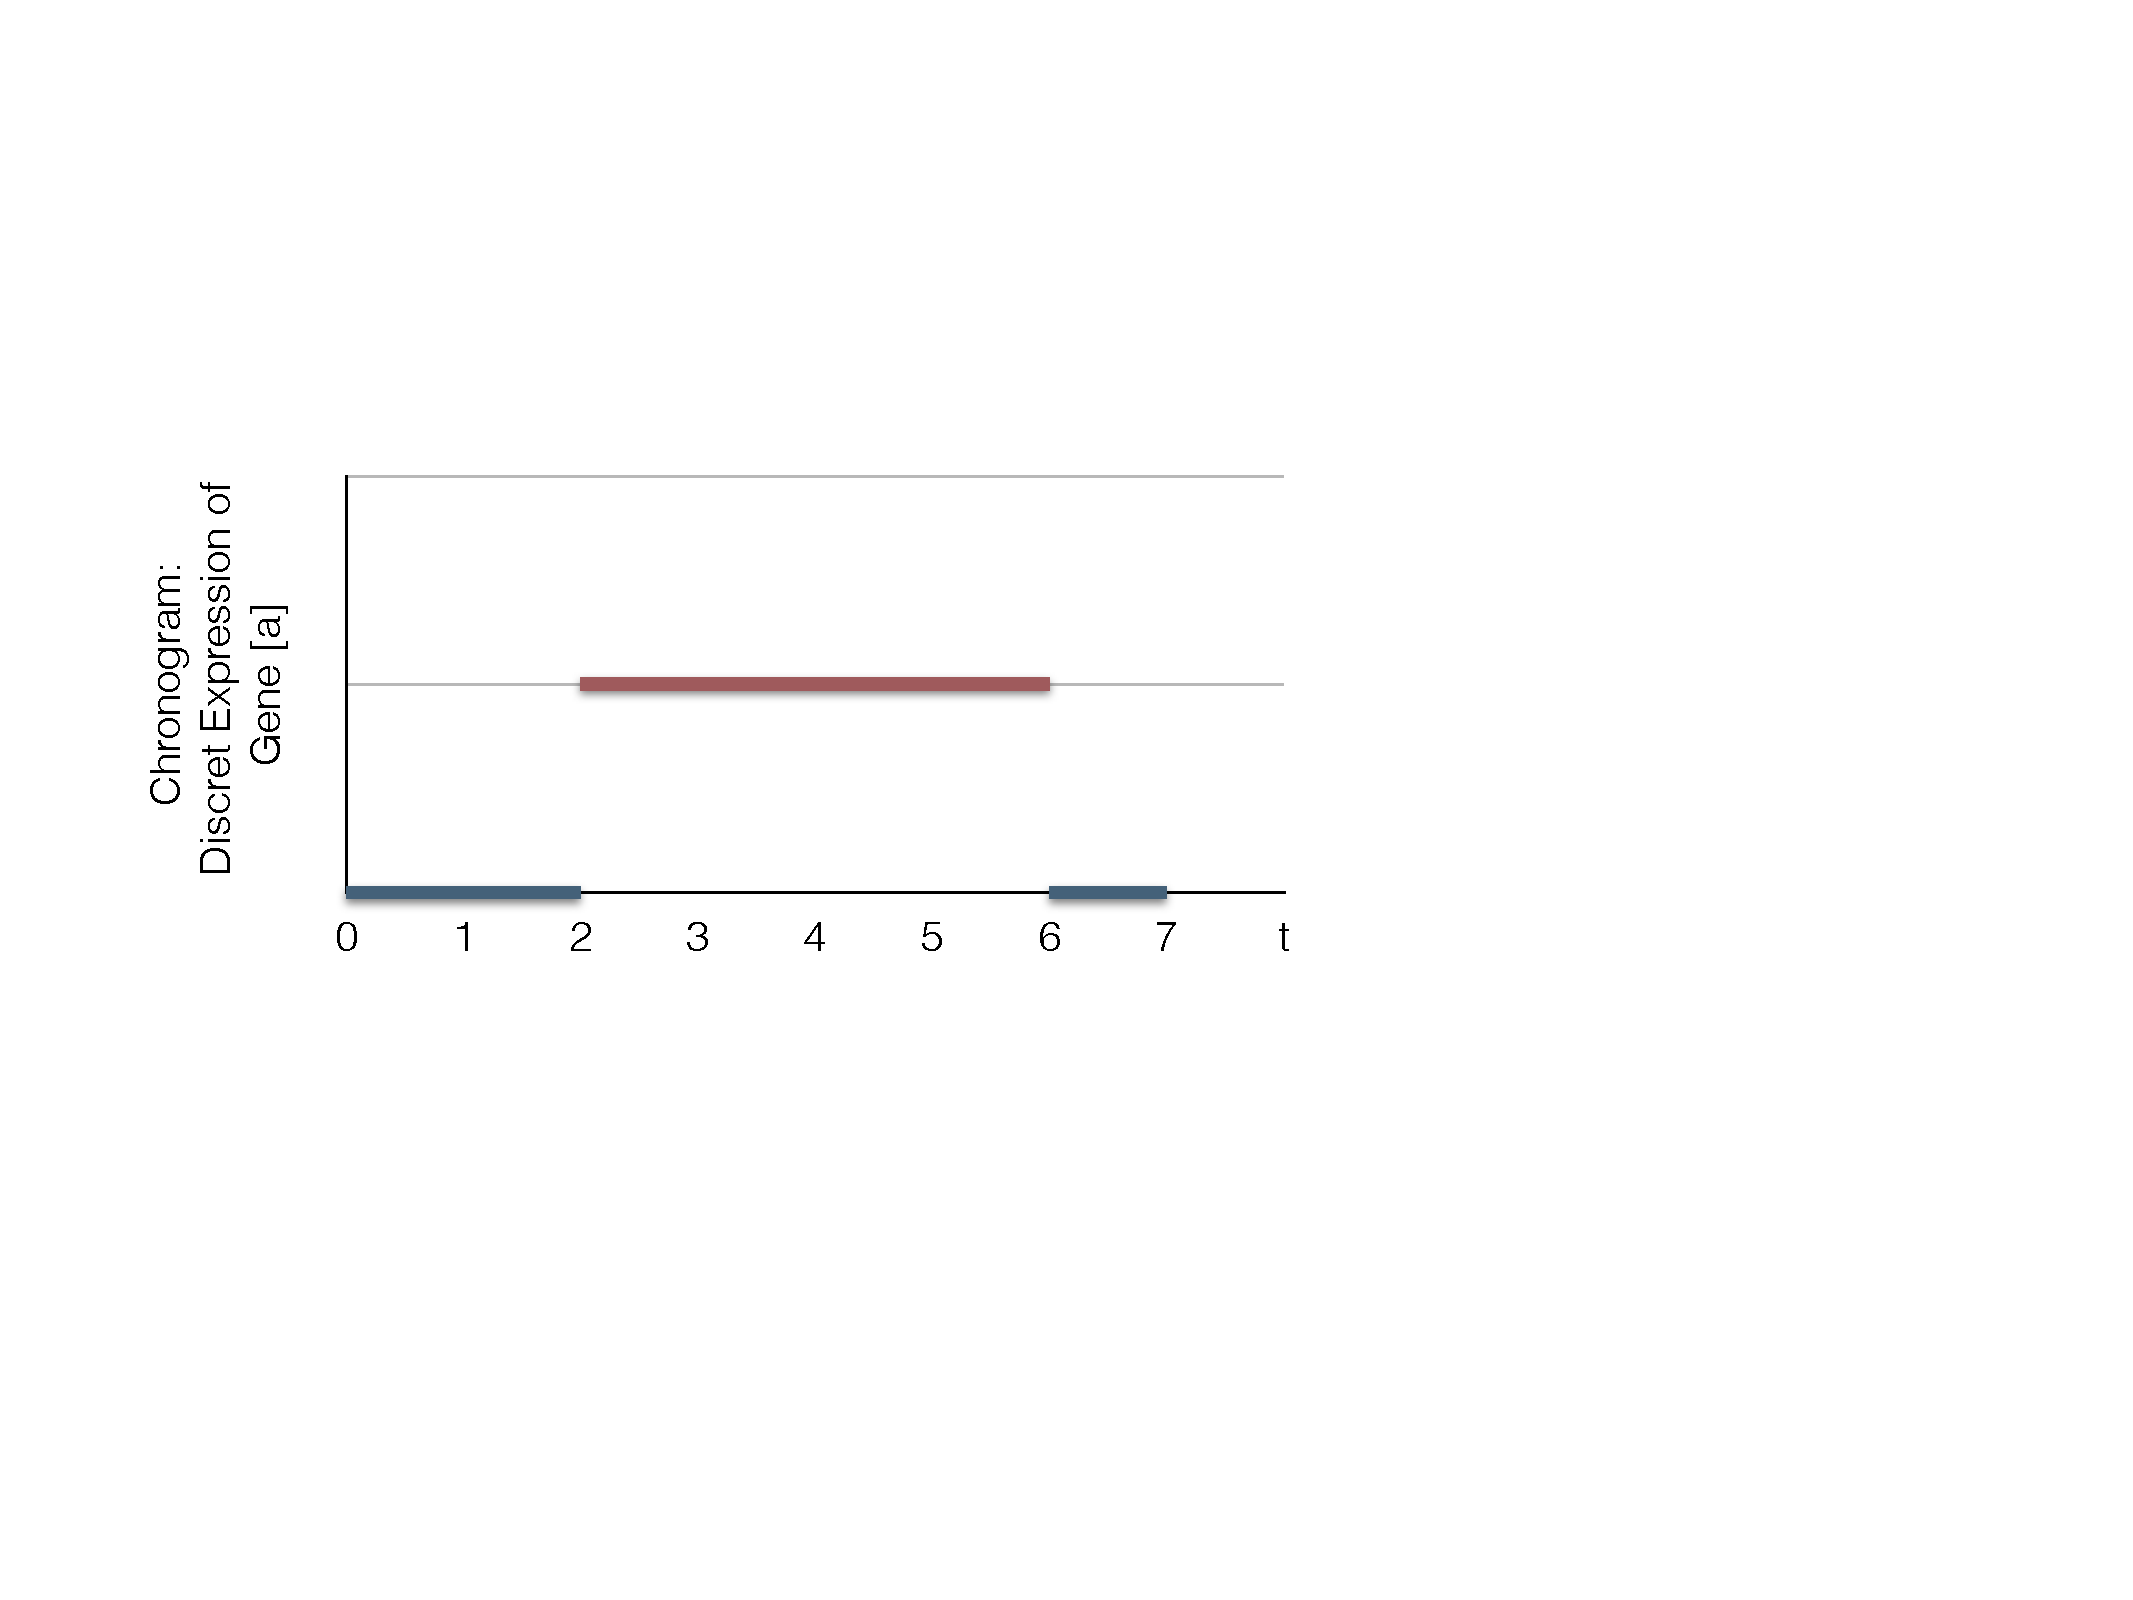
\includegraphics[ width =1\linewidth]{images/courbes/gene-z-disc.pdf}\\
\end{minipage}
\end{figure}